\documentclass{article}
\renewcommand\refname{Referencias}
\renewcommand\contentsname{\'Indice de Contenido}
\usepackage{graphicx}
\graphicspath{{../../IMG/}}
\usepackage{caption}
\usepackage{subcaption}
\usepackage{float}
\title{\textsc{Cuestionario N\'umero 1\\Inteligencia Artificial}}
\author{Ulises C. Ramirez}
\date{28 de Agosto, 2018}

\begin{document}
\maketitle
\newpage
\tableofcontents
\newpage
% === Inicio del cuerpo del documento. ===%
\section{Test de Turing}
\textit{\textsc{Consigna}: \textbf{Describa el test de turing. Fundamentos, Objetivos, Modalidades de Aplicaci\'on. Comentar, brevemente, los sitemas m\'as relevantes evaluados a partir del mismo en los \'ultimos a\~nos. ?`Qu\'e resultados han obtenido? ?`Se puede decir que el test haya sido superado?}}

A lo largo de la historia se siguieron cuatro enfoques cuando se habla de \textit{Inteligencia Artificial}, enfoques centrados en los \textit{humanos} y los centrados en la \textit{racionalidad} (Un sistema es racional si hace "lo correcto", en funci\'on de su conocimiento), a su vez podemos dividir estos en dos subgrupos, enfoques que hacen referencia a \textit{procesos mentales y al Razonamiento} y los que hacen referencia a la \textit{conducta}.

Entonces, si enumeramos el comportamiento que tendriamos seria de la siguiente manera:
\begin{enumerate}
\item Sistemas que piensan como humanos.
\item Sistemas que piensan racionalmente.
\item Sistemas que act\'uan como humanos.
\item Sistemas que act\'uan racinalmente.
\end{enumerate}

\subsection{Modalidades del Test de Turing}
La \textbf{prueba de Turing} seg\'un se postula en \cite{russel}  se dise\~no con el fin de proporcionar una definici\'on satisfactoria de inteligencia en vez de proporcionar una lista de cualidades necesarias para obtener inteligencia artificial, se sugiri\'o una prueba basada en la incapacidad de diferenciar entre entidades inteligentes indiscutibles y seres humanos. El test consiste en un di\'alogo con la m\'aquina, \textbf{si no es posible distinguir las respuestas del humano con las de la maquina, entonces, la m\'aquina es inteligente}. para lograr estas haza\~nas es necesario dotar al sistema con los siguientes atributos:
\begin{itemize}
\item Procesamiento del lenguaje natural.
\item Representaci\'on del conocimiento.
\item Razonamiento autom\'atico.
\item Aprendizaje autom\'atico.
\end{itemize}

Tambi\'en se puede hablar del \textbf{Test global de Turing}, la cual, ademas de probar que el sistema puede comportarse como un humano teniendo las capacidades que se mencionaron, permite evaluar la capacidad de percepci\'on e interacci\'on f\'isica del sistema mediante el intercambio de objetos f\'isicos entre el evaluador y el evaluado a trav\'es de una ventana, para lograr esto es necesario dotar a la entidad evaluada de lo siguiente:

\begin{itemize}
\item Visi\'on computacional.
\item Rob\'otica.
\end{itemize}



\subsection{Sistemas evaluados mediante el Test}


\subsection{Sobre la superaci\'on del Test de Turing}
Seg\'un se menciona en \cite{loebner2}, en Octubre de 2010, ante una docena de jueces, el concursante \textit{Elbot} se llev\'o el primer premio y acapar\'o los titulares de la prensa especializada gracias a su desenvuelto sentido del humor. Elbot enga\~no a 3 de los 12 jueces, y de haber enga\~nado a uno m\'as habria alcanzado el 30\% cifra que se considera como minimo para aprobar el Test de Turing.
Datos mas recientes, documentados desde el 2014 por \cite{loebner1}, sugieren que esta marca de 30\% no fue alcanzada, ademas de que las reglas como se comenta en \ref{sec:lp} establecen que se deben enga\~nar por lo menos a la mitad de los jueces. En las \'ultimas oportunidades que se celebr\'o la ceremonia, aunque a\~nos anteriores se tuvieron resultados prometedores, llegando a porcentajes de hasta 90\%, estos no representan la cantidad de jueces que fueron capaces de enga\~nar, m\'as bien la cantidad de preguntas que respondieron satisfactoriamente. Los datos mencionados se presentan en la secci\'on de Anexos \ref{sec:an1}.

\section{Loebner Prize}
\label{sec:lp}
\textsc{Consigna}: \textbf{Busca informaci\'on acerca de qu\'e es y para qu\'e se celebra el Loebner Prize}\\

Como se menciona en \cite{loebner1}, la sociedad dedicada a la Inteligencia Artificial m\'as grande del Reino Unido, en consonacia con otros articulos mencionados en la bibliograf\'ia tales como \cite{loebner2} \cite{loebner3}, el Premio Loebner es el concurso para el \textit{Test de Turing} mas viejo, iniciado en 1991 por Hugh Loebner y el Centro para Estudios del Comportamiento de la universidad de Cambridge.

\textbf{El concurso}: este consiste de 4 rondas donde en cada una, 4 jueces interactuar\'a con dos entidades usando un terminal, una de estas entidades sera un humando 'confederado' y el otro un sistema de Inteligencia Artificial. Despues de 25 minutos de interrogatorio el juez debe decidir cual de las entidades es el humano y cual es la IA. Si un sistema puede enga\~nar a la mitad de los jueves que es un humano, se le premia con una medalla de plata al creador de sistema.


\section{M\'etodos alternativos para la evaluaci\'on de la inteligencia de un sistema}
\textsc{Consigna}: \textbf{Con relaci\'on a la tem\'atica de la pregunta anterior, describa m\'etodos alternativos para la evaluaci\'on de la inteligencia de un sistema. Mencionar al menos dos sistemas de IA que en la actualidad puedan considerarse avanzados, describalos brevemente.}

\section{Chinese Room - \textit{J. R. Searle}}
\textsc{Consigna}: \textbf{Buscar informaci\'on acerca de la teor\'ia de la Habitaci\'on China que enunci\'o J. R. Searle en 1980. ?`En qu\'e consiste?}


Como se presenta en \cite{searle2009}, la Discusi\'on de la Habitación China busca refutar cierta concepcion del rol de la computaci\'on en el proceso humano para la adquisici\'on del conocimiento y el entendimiento a trav\'es del pensamiento, experiencias y sentidos.

El experimento va de la siguiente manera, como se expresa en un articulo publicado por el mismo \cite{searle1980}. Searle, se imagina a s\'i mismo solo en una habitaci\'on siguiendo ordenes de un programa de computadora para responder a caracteres chinos que se le pasan por debajo de la puerta. \'Este, no entiende nada de chino, y a\'un asi, siguiendo el programa para la manipulaci\'on de caracteres chinos, este puede producir cadenas de caracteres en chino que son apropiadas para as\'i enga\~nar a los que se encuentran fuera de la habitaci\'on y haerlos pensar que existe alguien que puede hablar chino dentro de la habitaci\'on, brevemente la conclusi\'on del argumento, es que \textit{programar una computadora puede hacer pareer que entiende el lenguaje, pero no tiene un entendimiento real}, por lo tanto, concluye que el Test de Turing no es aplicable \cite{cole2014}.

Esto se puede resumir de la siguiente manera, \cite{searle2009} postula que el argumento descansa sobre dos principios basicos enunciados por \cite{searle1980}:
\begin{enumerate}
\item ``Because the formal symbol manipulations by themselves don't have any intentionality; they are quite meaningless; they aren't even symbol manipulations, since the symbols don't symbolize anything. In the linguistic jargon, they have only a \textbf{syntax but no semantics}.''
\item ``Why on earth would anyone suppose that a computer simulation of understanding actually understood anything? It is sometimes said that it would be frightfully hard to get computers to feel pain or fall in love, but love and pain are neither harder nor easier than cognition or anything else. \textbf{For simulation, all you need is the right input and output and a program in the middle that transforms the former into the latter}. That is all the computer has for anything it does. To confuse simulation with duplication is the same mistake, whether it is pain, love, cognition, fires, or rainstorms.''
\end{enumerate}

\textbf{1. Sintaxis no es sem\'antica}: La sintaxis por si misma no es constitutiva de sem\'antica, tampoco garantiza la presencia de semantica por s\'i misma.

\textbf{2. Simulaci\'on no es duplicaci\'on}: Para poder recrear la cognicion humana en una m\'aquina no solamente ser\'ia necesario que simular el comportamiento humando, tambi\'en se tendria que duplicar los procesos cognitivos que dan cuenta del comportamiento que se trata de simular.


\section{Definici\'on propia de Inteligencia Artificial}
\textsc{Consigna}: \textbf{Defina con sus palabras qu\'e es la IA. Caracterice las l\'ineas de pensamiento en la presentacion de la teor\'ia, definiendo planteos de cada modelo.}

\section{Sistemas expertos conversacionales}
\textsc{Consigna}: \textbf{De los sistemas expertos conversacionales subidos como ejemplos. ?`Dentro de qu\'e categor\'ia lo clasificar\'ian? teniendo en cuenta el an\'alisis de las diferentes definiciones sobre inteligencia artificial.}

\section{?`Qu\'e entiende por ense\~nar y aprender?}

\section{Problemas o \'Ambitos de Aplicaci\'on de la IA}
\textsc{Consigna}: \textbf{Caractericec los problemas o \'ambitos de aplicaci\'on principales de la IA. Releve t\'ecnicas aplicables en la actualidad y ejemplificque usos en los \'ultimos a\~nos que considere casos de \'exito.}

\section{An\'alisis de definici\'on}
\textsc{Consigna}: \textbf{Analice la siguiente definici\'on e indique cuales son los aspectos que sobresalen en ella: \textit{La inteligencia artificial estudia como lograr que las maquinas realicen tareas que, por el momento, son realizadas mejor por los seres humanos}.}

\section{Conocimiento/Informaci\'on}
\textsc{Consigna}: \textbf{?`Conocimiento es sin\'onimo de informaci\'on? Analice el siguiente ejemplo: Si A es verdadero entonces B es verdadero, Sino C es falso.}

\section{?`Qu\'e caracter\'isticas debe tener un problema para aplicar t\'ecnicas de IA?}


\section{Anexos}
\subsection{Datos Premio Loebner}
\label{sec:an1}
A continuaci\'on se listan los resultados de diferentes a\~nos para el Premio Loebner, extra\'idos de \cite{loebner1}.
\begin{figure}[h]
\centering
\begin{minipage}{.5\textwidth}
  \centering
  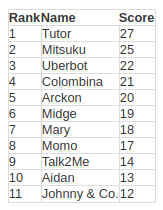
\includegraphics[width=.4\linewidth]{TT2018}
  \captionof{figure}{Resultados 2018}
  \label{fig:tt2018}
\end{minipage}%
\begin{minipage}{.5\textwidth}
  \centering
  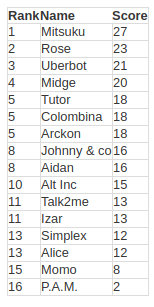
\includegraphics[width=.4\linewidth]{TT2017}
  \captionof{figure}{Resultados 2017}
  \label{fig:tt2017}
\end{minipage}
\end{figure}

\begin{figure}[H]
\centering
\begin{minipage}{.5\textwidth}
  \centering
  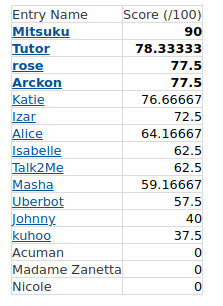
\includegraphics[width=.4\linewidth]{TT2016}
  \captionof{figure}{Resultados 2016}
  \label{fig:tt2016}
\end{minipage}%
\begin{minipage}{.5\textwidth}
  \centering
  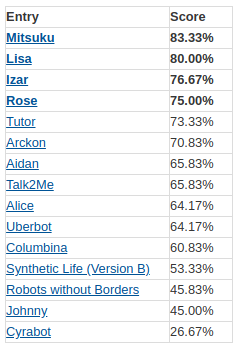
\includegraphics[width=.4\linewidth]{TT2015}
  \captionof{figure}{Resultados 2015}
  \label{fig:tt2015}
\end{minipage}
\end{figure}

\begin{figure}[H]
  \centering
  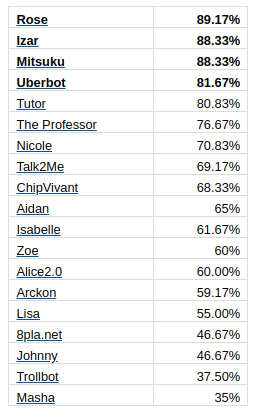
\includegraphics[width=.4\linewidth]{TT2014}
  \caption{Resultados 2014}
  \label{fig:tt2014}
\end{figure}\\
\newpage
% ==========Bibliografia===================================

\begin{thebibliography}{9}
	% Item 1
	\bibitem[Russel y Norvig, 2004]{russel}
	\newblock \textsc{Russel, S. J.; Norvig, P.} \textit{Inteligencia Artificial, Un Enfoque Moderno}. Pearson Educaci\'on, S.A., Madrid, 2004, \textsc{ISBN: 84-205-4003-x}
	% Item 2
	\bibitem[Gonz\'alez, 2007]{gonzalez2007} \textsc{Rodrigo Gonz\'alez}. \textit{El test de Turing: dos mitos, un dogma}. Katholieke Universiteit Leuven, 2007, \textsc{doi: 10.4067/S0718-43602007000100003}
	% Item 3
	\bibitem[AISB]{loebner1} \textsc{The Society for the Study of Artificial Intelligence and Simulation of Behaviour}. \textit{Loebner Prize}. AISB. https://www.aisb.org.uk/events/loebner-prize [Consultado el 4 de Septiembre, 2018]
	% Item 4
	\bibitem[VA, 2010]{loebner2} \textsc{Varios autores}. \textit{El test de Turing en su m\'axima competici\'on: Loebner Prize}. System and Software Engineering, 2004. http://www.gtd.es/es/blog/el-test-de-turing-en-su-maxima-competicion-loebner-prize [Consultado el 4 de Septiembre, 2018]
	% Item 5
	\bibitem[Moloney, 2017]{loebner3} \textsc{Charlie Moloney}. \textit{How to win a Turing Test (the Loebner Prize)}. Chatbots Magazine, 2017. https://chatbotsmagazine.com/how-to-win-a-turing-test-the-loebner-prize-3ac2752250f1 [Consultado el 4 de Septiembre, 2018]
	% Item 6
	\bibitem[Cole, 2014]{cole2014} \textsc{David, Cole}.\textit{The Chinese Room Argument}. The Stanford Encyclopedia of Philosophy (Winter 2015 Edition), Edward N. Zalta (ed.), https://plato.stanford.edu/archives/win2015/entries/chinese-room [Consultado el 5 de Septiembre, 2018]
	% Item 7
	\bibitem[Searle, 2009]{searle2009} \textsc{John, Searle}.\textit{Chinese room argument}. Scholarpedia, 4(8):3100. http://dx.doi.org/10.4249/scholarpedia.3100 [Consultado el 5 de Septiembre, 2018]
	% Item 8
	\bibitem[Searle, 1980]{searle1980} \textsc{John, Searle}. \textit{Minds, Brains and Programs}, Behavioral and Brain Sciences, 3: 417-457, http://cogprints.org/7150/1/10.1.1.83.5248.pdf
\end{thebibliography}

\end{document}
